\documentclass{standalone}
\usepackage{tikz}
\usetikzlibrary{decorations.pathreplacing}
\usepackage{amsfonts}


\begin{document}
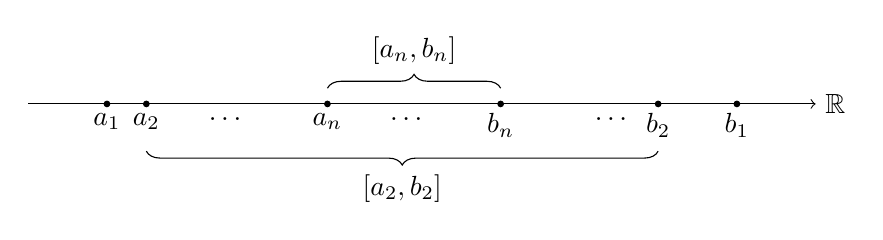
\begin{tikzpicture}
% Draw the real line
  \draw[->] (-5,0) -- (5,0) node[right] {$\mathbb{R}$};
  
  % Draw the point 'x' and '0'
  \filldraw (-4,0) circle (1pt) node[below] {$a_1$};
  \filldraw (4,0) circle (1pt) node[below] {$b_1$};


   \filldraw (-3.5,0) circle (1pt) node[below] {$a_2$};
  \filldraw (3,0) circle (1pt) node[below] {$b_2$};  
  
  
   \filldraw (-1.2,0) circle (1pt) node[below] {$a_n$};
  \filldraw (1,0) circle (1pt) node[below] {$b_n$};  
  
  
  % Draw dots
  \draw (-2.5,0) node[below=1.5pt] {$\ldots$};
  \draw (2.4,0) node[below=1.5pt] {$\ldots$};
  \draw (-0.2,0) node[below=1.5pt] {$\ldots$};
  
  \draw[decorate,decoration={brace,amplitude=5pt}] (-1.2,0.2) -- (1,0.2) node[midway,above=5pt] {$[a_n,b_n]$};
  
  \draw[decorate,decoration={brace, mirror, amplitude=5pt}] (-3.5,-0.6) -- (3,-0.6) node[midway,below=5pt] {$[a_2,b_2]$};
  
  
  \end{tikzpicture}
\end{document}